\documentclass[11pt, a4paper]{article} % , draft
\usepackage[utf8]{inputenc}

\usepackage{enumitem} % customiçe item dots etc
\usepackage{textgreek} % obv
\usepackage{physics} % for easy derivative notation
\usepackage{amsmath}
\usepackage{amsthm} %theorems
\usepackage{amssymb}
\usepackage{mathtools} % for matrices with blocks inside
\usepackage[scr=boondoxo]{mathalfa}
\usepackage{pst-node}%
\usepackage{mathrsfs}
\DeclareMathAlphabet{\mathpzc}{OT1}{pzc}{m}{it}

\newcommand{\mc}{\multicolumn{1}{c}}
\newcommand{\R}{\mathbb{R}} % command for real R
\newcommand{\Holo}{\mathcal{H}}
\newcommand{\M}{\mathcal{M}}
\newcommand{\C}{\mathbb{C}}
\newcommand{\N}{\mathbb{N}}
\newcommand{\z}{\mathpzc{s}}
\newcommand{\p}{\mathpzc{r}}
\newcommand{\s}{\mathbb{S}}
\newcommand{\W}{\mathbb{W}}
\newcommand{\U}{\mathscr{U}}
\newcommand{\Lg}{\mathscr{L}}
\newcommand{\x}{\mathcal{X}}

\usepackage{csquotes}
\MakeOuterQuote{"}
\setlength{\parskip}{0.3 cm}

\usepackage{fancyhdr}

%\usepackage{nath} % authomatic parenthesis stuff
%\delimgrowth=1
\usepackage[left=2cm, right=2cm, top=2.1cm, bottom=2.1cm]{geometry} % set custom margins
\usepackage{graphicx} % to insert figures
\usepackage{grffile}
\graphicspath{{Figures/}} % define the figure folder path
\usepackage{subcaption} % for multiple figures at once each with a caption
\usepackage{multirow} %multirow in tables

\usepackage{caption}
\captionsetup[figure]{font=footnotesize} %adjust caption size
\captionsetup[table]{font=footnotesize} %adjust caption size

\usepackage{booktabs} % for pretty tabs in tables
\usepackage{siunitx} % Required for alignment
\captionsetup{labelfont=bf} % bold face captations

\usepackage{hyperref} % makes every reference a hyperlink
\hypersetup{
    colorlinks=true,
    linkcolor=violet,
    filecolor=[rgb]{0.69, 0.19, 0.38},      
    urlcolor=[rgb]{0.0, 0.81, 0.82},
    citecolor=[rgb]{0.69, 0.19, 0.38}
}

\usepackage{epigraph} % for quotations in teh begginig
\setlength\epigraphwidth{8cm}
\setlength\epigraphrule{0pt}
\usepackage{etoolbox}
\makeatletter
\patchcmd{\epigraph}{\@epitext{#1}}{\itshape\@epitext{#1}}{}{}
\renewcommand{\qedsymbol}{o.\textepsilon.\textdelta}

\newtheorem{prop}{Proposition} %so I can use propositions
\newtheorem{cor}{Corollary} %so I can use corollaries
\newtheorem{defi}{Definition} %so I can use corollaries

\makeatother % all this is for the epigraph
\usepackage{tocloft}

\usepackage{imakeidx} % make index

\makeindex[columns=3, title=Alphabetical Index, intoc]

%\title{\vspace{-2.5cm} {\bf Can we make the Exponential scaling in Time\\ be Linear in Time if Parallelized Exponentially? \\ {\em - Part 2 -}} \vspace{-0.4cm}  }
\title{\vspace{-2cm} {\bf An Intuitive Narrative for\\ Open Quantum Systems?}\\{\small by {\em Xabier Oyanguren Asua}}\vspace{-0.8cm}}
\date{\vspace{-11ex}}
\let\clipbox\relax
\usepackage{adjustbox}
\newcolumntype{?}{!{\vrule width 1.5pt}}
\usepackage{abstract}
\setlength{\absleftindent}{0mm}
\setlength{\absrightindent}{0mm}

\usepackage{tcolorbox}
\DeclareRobustCommand{\mybox}[2][gray!10]{%
\begin{tcolorbox}[   %% Adjust the following parameters at will.
        left=0.2cm,
        right=0.2cm,
        top=0.15cm,
        bottom=0.15cm,
        colback=#1,
        colframe=#1,
        width=\dimexpr\textwidth\relax, 
        enlarge left by=0mm,
        boxsep=5pt,
        arc=0pt,outer arc=0pt,
        ]
        #2
\end{tcolorbox}
}


\usepackage{anyfontsize}

\NewDocumentEnvironment{kapituloBerria}{mm}
{\clearpage           % we want a new page          %% I commented this
   \thispagestyle{empty}% no header and footer
   \vspace*{\stretch{2}}% some space at the top
   \raggedleft          % flush to the right margin
   {\textbf{{\fontsize{60}{40}\selectfont \hspace{+9.5cm}#1 \newline \newline}}}
   \bf
   \fontsize{30}{20}\selectfont
  }
  {\par % end the paragraph
   \vspace{\stretch{3}} % space at bottom is three times that at the top
   \normalfont
      \fontsize{15}{20}\selectfont
      \vspace{-1cm}
   \begin{flushleft}{ \textit{#2}  }
   \end{flushleft}
   \clearpage           % finish off the page
  }
  
%\newenvironment{kapituloBerria}[2]
  

\usepackage{listings}
\usepackage{xcolor}
\lstset{language=C++,
                basicstyle=\ttfamily,
                keywordstyle=\color{blue}\ttfamily,
                stringstyle=\color{red}\ttfamily,
                commentstyle=\color{green}\ttfamily,
                morecomment=[l][\color{magenta}]{\#}
    backgroundcolor=\color{black!5}, % set backgroundcolor
    basicstyle=\footnotesize,% basic font setting
}

\begin{document}

\clearpage
%% temporary titles
% command to provide stretchy vertical space in proportion
\newcommand\nbvspace[1][3]{\vspace*{\stretch{#1}}}
% allow some slack to avoid under/overfull boxes
\newcommand\nbstretchyspace{\spaceskip0.5em plus 0.25em minus 0.25em}
% To improve spacing on titlepages
\newcommand{\nbtitlestretch}{\spaceskip0.6em}
\pagestyle{empty}
\begin{center}
\bfseries
\nbvspace[1]
\Huge
{\nbtitlestretch\huge
AN INTUITIVE NARRATIVE FOR\\
OPEN QUANTUM SYSTEMS?
}

\nbvspace[1]
\normalsize

TOWARDS A NARRATIVE TO \\
MAKE QUANTUM MEASUREMENTS\\ 
AND OPEN SYSTEM DYNAMICS\\ INTUITIVE \\

\nbvspace[1]

Drafting a Quantum Intuition\\
that minimizes unjustified assumptions

\nbvspace[1]
\small BY\\
\Large Xabier Oyanguren Asua\\[0.5em]
%\footnotesize Can we really foresee the future of the Universe?"\\


\nbvspace[6]


\includegraphics[width=2.5in]{UAB.png}
\normalsize
\vspace{-0.5cm}
%\small Thesis Directors: \\
%\nbvspace[0.2]
%\large Jordi Mompart Penina \\
%Xavier Oriols Pladevall\\
%\nbvspace[1]

%Universitat Autònoma de Barcelona\\
\large
%DEGREE FINAL DISSERTATION \\
\small
%Bachelor's degree in Nanoscience and Nanotechnology \\
\small
$\ $Winter 2021-2022
\nbvspace[1]
\end{center}
\newpage
\null
\clearpage

\maketitle
\pagenumbering{gobble}
\setlength{\cftbeforesecskip}{0.4cm}
\setlength{\cftbeforesubsecskip}{0.4cm}
\setlength{\cftbeforesubsubsecskip}{0.25cm}

\tableofcontents
\clearpage
\pagenumbering{arabic}
\setcounter{page}{0}
\vspace{-0.3 cm}

\pagestyle{empty}

\section*{Abstract}


\section*{Objectives}\vspace{-0.2cm}



\section*{Guideline}\vspace{-0.2cm}


\newpage
\pagestyle{fancy}
\fancyhead[L]{Philosophical Prolegomena}
\fancyhead[R]{\em On the Nnoumenon and Phenomenon}

\section*{\centering \huge{Philosophical Prolegomena}} %Preface
\addcontentsline{toc}{section}{Philosophical Prolegomena}
\subsection*{On the Noumenon and Phenomenon}
\addcontentsline{toc}{subsection}{On the Noumenon and Phenomenon}

Focus your attention for a moment in that thing that is behind the eyes that are reading these lines and in front of the back of your head. Perhaps a bit upper than the eyes. There, in the center of your "world" or reality. We call it {\bf consciousness}. It is you, the light that makes you. That thing that when a person expels the last breath, is no longer there \footnote{It is no longer there when you are deep asleep either...}. That thing that when you look at the eyes of another person, you are (or at least expect to be) looking at. The relevance of that thing, the self-aware consciousness, is the following. Imagine you discover that the reality you considered as true and contingent and objectively material, is actually fake. For example, that your brain is actually in a liquid tank in some lab and it has connected to its visual-, auditive-, self-body internal perceptive- etc. cortices or brain regions, some electrodes that stimulate the exact same neural pulses that would be stimulated by a true perception in the visual neurons of a human eye that could be reading this, tactile neurons that could be wearing those clothes or internal nerves that would feel the body extension you feel. Well, there is absolutely no way to prove that this is not indeed the case. No way. Thus, there is no way either to prove that behind the eyes of the rest of the people there is a consciousness like yours. There is actually no way either to prove that your brain was not spontaneously arranged in the vacuum of space due to statistical fluctuations with these exact memories and current perceptions. Not either that it is not the product of a super-computer simulating each and every electron and fundamental particle in your brain to the quantum level, with these cortices being activated according to the algorithm of the machine, to make you feel this reality. There is no way either, in this line, to know that this consciousness should have any sort of ontologically material cause or foundation. \vspace{-0.3cm}

So yeah, everything could simply be "fake". Well, everything, except for one thing: that {\em you}, that light of self-awareness that is behind those eyes, that, which we call {\em you}, exists. The fact that {\em you} exist is necessarily true for you. It needs no prove, because from the moment in which you are able to think, its existence is a necessity. Pause and ponder it for a moment, and realize about its trueness. We are not talking about the rest of humanity, just you, in your awareness. The rest of humans could also be fake together with the perceptual reality you are placed in. But as long as you "think", you are: you exist. No possible discussion about it. {\em "Cogito ergo sum"}, I think, therefore I am, Descartes' famous statement.

Great, so now we are both on the same beginning of the story. Let us call that "self-aware-conscious-light" that is currently reading this, simply as "the {\em cogito}".

Now, lets make explicit the first assumption or postulate that any human being makes everyday: there exists an objective and materially contingent external reality, in which your {\em cogito} is placed as a cursor in a stage. Your {\em cogito} doesn't know directly about this scenario, else the stage itself would be part of the same mind. Instead, your {\em cogito} is attached to some organic sensors, like the neurons in your eardrum, which get activated in different ways according to how the external reality modulates the shape of the eardrum membrane. Accordingly it generates a signal that the neurons send to the acoustic cortex or region in your brain. The same happens for some visual neurons that are excited in different ways as a function of the energy of the light arriving to them etc. The same for the olfactory, gustatory, tactile, accelerometric (the inner ear liquid that lets you know the direction of gravity) or proprioceptive nerves\footnote{Proprioception is the information we receive from muscles, tendons and joints that allow us to know where our body parts are at any given moment even if we close our eyes.}. Once all this information arrives to the brain, it is processed and each chunk is projected as perceptual feelings surrounding the center of your person, around your {\em cogito}. As such, the particular colors, tastes, sounds etc, you will feel are generated in that processing, presumably due to specific excitations in the sensor organs\footnote{Think about how unique those projections you feel are, that you will never be able to know if what you "see" and call "red" is not seen by another person as what you call "blue", just that you both agree it is called "red".}. Let us give these concepts some names: the "external" reality to your {\em cogito}, the reality "in itself", the one you will never know about, because you can only know through your perceptual sensors, is called {\em \bf noumenon} (assuming of course, that such a thing objectively exists with the same certainty as your own {\em cogito}). Meanwhile, the set of projections where your {\em cogito} is centered, all that "virtual" surrounding that the processing of your perceptions produces around your {\em cogito}, is called the {\em \bf phenomenon}. Of course, it is also convenient to accept the hypothesis that not only there is an objective {\em noumenon}, but that the rest of people have also behind those eyes, their own {\em cogito}, and that those {\em cogito}-s are also centered at a {\em phenomenon}, which is at least very similar to yours.

Now, note that what you know about the "external" reality is necessarily restricted to the particular way in which it is projected in your {\em phenomenon}! That is, about this {\em noumeno}, you will never know anything that cannot be directly or indirectly sensed and represented into your phenomenon. We are imprisoned in our phenomena. To convince you even more about the tangential nature of the {\em phenomenon} and {\em noumenon}, let me remember you that whenever you are dreaming, you see and touch things or even feel your own body in configurations, that are really "not true". Your brain is generating directly in the visual, auditive and other cortices, the same neuronal excitations that would be generated if your eyes received that light, or your arms were in that disposition, when in reality your eyes are closed and your arms are still hugging your teddy bear. So yeah, dreaming is indeed the most immersive of the virtual realities. If you had a computer stimulating those regions with those same pulses, you would feel the same projections in the phenomenon. Dreaming just has the little inconvenience that the reasoning cortex is at least partially inhibited (together with the motor cortex -the one making your body actually move). That is why you feel more "instinctive" and less aware, like if your judgment was covered in a sort of veil. That is why you never confuse the oneiric- with the daylight- phenomenon. Clearly, if you made the inhuman experiment to avoid the rational cortex to be inhibited, you would entirely feel a dream, as real as right now, following the fact that if you avoid the inhibition of the motor cortex you will move in the reality as you are moving in the dream. Of course, "the plot"  of that reality would be certainly confusing and inconsistent, like for Alice was the Wonderland, but the pehnomenon in itself would feel material. Think about it.\vspace{0.3cm}

\mybox{ {\bf Extra Thoughts: Solipsism, Antropocentrism and a Cosmic Logos \\ \centerline{-The Arithmetic Paradox-} \vspace{-0.2cm}  \\ }
All this can easily lead you to {\em solipsism}, the philosophical posture where {\em you} are the only existing one, and as such, the reason of existence for all of your perceptions is your own existence. That is, {\em esse est percipi}, or whatever that {\em is}, can only {\em be}, if and while it is perceived by your {\em cogito}. That is, the Universe is as long as, or where, your {\em cogito}'s light illuminates it. That is, the Universe does not manifest its existence by itself. Instead, its "real"-ity is only as long as your {\em cogito} lights it. But sure, if you have accepted the postulate that there is such a thing as a {\em noumenon} (which you provide with existence through your phenomenon), why not accept also that there are more {\em cogito}-s lighting more {\em noumena}?\vspace{-0.2cm}  \\

At this step, you may realize that there is apparently a common {\em noumenon} for all of those {\em cogito}-s, because, the rest of {\em cogito}-s seem to report changes in their phenomena that are identifiable with changes in your own phenomeon. It is this inter-personal agreement of coherence why we know dreams are not reality. Dreams do not alter this "common" {\em noumenon}. Only {\em you} feel the oneiric phenomenon. Schrödinger tries to manifest this dilemma in his {\em Mind and Matter} with the name "Arithmetic Paradox": How can there be multiple cogito-s, each giving existence with its light to the representations projected in each individual phenomenon, but even so, exist a single and shared {\em noumenon}?\vspace{-0.2cm} \\

Realize how the problem of this reality that requires to be part of a {\em phenomenon} for its existence to be manifested, but where not all the Universe is perceived by somebody at all times, could be solved by a rather simple idea.}

\mybox{ The existence in itself of the Universe could be guaranteed without the need of having us, mammals, so casual results of evolution, which could have simply never come to live, by imagining a cosmic {\em cogito} that makes everything be explicitly manifested at all times. A {\em cogito} projecting the phenomenon of all the Universe at all times, and thus alleviating our fear of our Universe being a void theater if we were not here. We could identify this cosmic {\em cogito} with the pre-established harmony of Leibniz, perhaps a justified pretext for a greater existence or perhaps just the master algorithm that connects the perceptions that the computer simulating our brains needs to take care of. On this last idea, note that if we wanted to simulate a bunch of human brains -assuming a {\em cogito} can really emerge from non-organic computations- and make them believe they are "real" we would only need to simulate the atoms of their brains and the neural pulses generating their phenomenon, with the boundary condition of letting the different phenomenons influence each other. No need to simulate the whole Universe to make them believe they are true. \vspace{-0.2cm} \\

Notice however, before sanctifying the cosmic {\em cogito}, mother algorithm or pre-established harmony, that its existence is just one possible exit for the {\em impasse} of the arithmetic paradox over solipsism. We should never forget that the first lesson is ones {\em cogito} and that all the rest of concepts are based on postulates that build up one after the other over ones {\em cogito}. If suddenly a postulate of these erases the need of having the {\em "cogito ergo sum"} as basis for the existence, then that is cheating the argumentation. Beneath this hypothesis, there will always be the one and only undeniable true that needs no prove: {\em you exist}. Yeah, perhaps it is too anthropocentric. But it seems to be the least arbitrary and least unjustified conviction a human being could have.
}

Then, just realize that how {\em we} perceive sound or images or any other perception, is due exclusively to how our human brains process the information and manifest their corresponding projections on the phenomenon. That is, if there could be other {\em cogito}-s, evolved in different circumstances, they could have a different phenomenon to ours in front of the same stimuli or same {\em noumenon}. As an example, we know that dogs for instance, have a smaller variety of visual sensor neurons and thus end up having a phenomenon with a bi-chromatic range (they "see" in gray-scales). Now, let us call the rules that make us manifest the projections in the particular ways we do (or dogs do) as mental {\em \bf categories}. These include two kinds: the purely perceptual ones -the axioms of raw perception- and the cognitive ones -the axioms of abstraction and comprehension-. 

The \textbf{perceptual categories} are those that map, for instance, certain light energies to certain colors, certain frequencies of air oscillations to certain perceived sounds or certain kinds of molecules to certain smells. If one was to explain to a non-human intelligence what music is, would need to resort to these.

Then, there are the \textbf{cognitive categories}, that are the basic essences through which we think and understand things (and through which we are doomed to understand them, as certainly as we are doomed to undeniably feel our own existence). For example, the idea of "unity" (of "one") as a concept, of "existence", or even "boundedness", which might be derived from having the idea of "unity" and "non existence" at the same time. These at the same time imply the category of "fragmentation": the reason why when you look at a scene you are able (and doomed to do so) of seeing and understanding individually delimited and separated things, as if they had independent existence from each other. You do not see everything as a single continuum, even if in the noumenon it could be that it is so. As a taste of how the nomenon could in fact be incompatible with the "fragmentation", notice that "physics" is essentially the study of the best model about the {\em noumenon} we can build, the best story to explain and predict the behavior of the {\em noumenon} and its consequences in the phenomenon. If our current models are good enough representations of the noumenon, then we know that in reality matter is a continuum of atoms that make really no distinction of whether they belong to a chair, to this paper or your own body, meaning that our "fragmentation" category is just the way we understand things, not something fundamental about reality. Most importantly however, these cognitive axioms are in essence, where mathematics are rooted on, the axioms that build them.

\subsection*{On Models, Interpretations and Narratives}
\fancyhead[R]{\em On Models, Interpretations and Narratives }
\addcontentsline{toc}{subsection}{On Models, Interpretations and Narratives}
\begin{flushright} \em "Being able to predict reality, does not make you understand it."
\end{flushright}

We can define a {\bf physical model} or {\bf theory}, as a mathematical construction that allows the prediction of reality (that is, of the events happening on the phenomenon).

A physical model must have two elements. One is a {\bf mathematical model}, which is a self-consistent mathematical construction. The other one is a {\bf basic interpretation} of the mathematical model, which can be defined as a set of links established between the mathematical entities of the model with phenomenological qualities that appear in our perceptions.

Now, such a physical model or theory, is enough from an operational point of view. It is enough for predicting the events we can perceive, which from an utilitarian view, is all physics should be about. However, we humans, have a natural tendency towards not only building physical models, as utilitarian mathematical tools, but for also seeking semantical or narrative models about reality. Stories that can aid us conceptually and intuitively understand what could be happening in the noumenon for the model to correctly predict the events we find in the phenomenon. We can define an {\bf interpretation} or {\bf narrative} of a physical model, as a self-consistent semantic story given to the mathematical structures and elements of the theory, that go beyond the set of concepts anchored to the phenomenon by the basic interpretation we defined earlier. That is, it is a conceptual representation of the noumenon, beyond the phenomenon. A conceptual representation that is consistent with each mathematical step given in the base physical model. 

The fact that physical models or theories only speak about phenomoenological events, qualities we immediately perceive, make them falsifiable. If a certain model fails in some prediction, the model will be false for a general case. However, interpretations or narratives talk about the noumenon, which by definition is "the external reality in itself, without us perceiving it through our senses and categories". This noumenon thus can never be known in itself, it is epistemologically inaccessible. Therefore, as long as a narrative is consistent with the mathematics of the model, it will be unfalsifiable as a model for the noumenon. This is, as long as the physical model it is grounded on is not proven to be incorrect.

It is this why one could say that working on an interpretation for a physical theory is a useless task. And it is indeed, from a purely productive or utilitarian point of view. However, since being able to predict reality does not make you understand it, there is place for scientists working on narratives. Intuitively understanding a theory, does not only allow a person to better make the questions about the model that can pull it to its limits, but it is also a way to better make it understand it, remember it and use it. Just as learning a text as part of a song makes it easier to digest it, or a moral is simpler to take when first known about through a tale, so is the case for a physical theory with a simple narrative, rather than the naked basic interpretation. It is a task that might not be as creative as creating the physical model itself, but is at least as imaginative and coloring for the community that reaches it. We could compare the physical theory with the outline of a picture, which has to be created "out of nothing", and thus has a big creative merit, while we could compare the interpretation or narrative with the coloring of the outlined picture. The painter is not "creating nothing usefully new", but, it gives body, consistency, appeal and digestibility to the overall picture.

In the present dissertation an illustrative narrative for the physical model comprehended under the name "Non-Relativistic Quantum Mechanics" will be exposed, as a means of introducing an intuitive explanation of the so called Open Quantum systems and their quandary.




\newpage


\begin{kapituloBerria}{Part A}{" Quantum Mechanics is Ontologically\\ Deterministic but Epistemologically Stochastic."}
The Axioms 
\end{kapituloBerria}
\newpage
\fancyhead[L]{\null}
\fancyhead[R]{\null}
\null
\clearpage


\section*{\centering \huge{Part A: The Axioms}\vspace{-0.3cm}}
\noindent\rule{\textwidth}{0.4pt}

{\bf Axioms} are the principles or assumptions from which the understanding of something is built up. They are principles that are rather unprovable or self-evident and are admitted as the first facts in the deductive creation of a conceptual framework. This means that if one keeps on asking $why?$ within a certain framework, the last answers one can arrive to are these axioms over which all the rest is formulated. \vspace{0.2cm}

\mybox{As an example, the following ones are some of the main axioms of physics (here, axioms may also be called {\bf postulates}):\vspace{-0.1cm}
\begin{itemize}
\item The postulate that the {\em noumenon}, or at least its consequences in our {\em phenomenon}, are understandable for human cognition.\footnote{Note how this is a rather arbitrary assumption (as most axioms are). The inner workings of reality could have also been incomprehensible for human cognition! Yet, till date it looks like the Universe is understandable. } 

\item The postulate that this understandability, these rational models, can be formalized mathematically as a particular example of some mathematical construct, building what we called a physical model or theory in the preface.

\item The postulates that fix the degrees of freedom of these physical models to fit our phenomenologic observations. These are postulates about some direct or indirect experimental observations we find in the phenomenon: for example, the Planck constant is this particular number because we see/measure it to be so, or time is absolute or not because we experimentally see so etc.\vspace{-0.1cm}
\end{itemize}

It is interesting to note that in maths on the other hand, the axioms are the {\em cognitive categories} we talked about in the prologue: unity, fragmentation, inclusion, boundedness etc. The mental categories that shape our mind. Most importantly, note that there are no experimental postulates in mathematics. This is the reason why mathematics needs no experimental proof, and no matter how complicated a mathematical theory is, once one understands the formal proof, its trueness is obvious and self-evident. This is because in its last resort, a mathematical statement is built on fundamental concepts with which you are doomed to understand the Universe (the cognitive categories). You are inevitably tied to those concepts as well as you are tied to your own existence by the {\em cogito ergo sum}.}

Much in the same way, a narrative of a physical model, also has axioms or basic assumptions. Even if in general these are not explicited, it is a very interesting point to begin from, since these are the loose ends of the interpretation. 

In this first part of the document, we will delve with the basic postulates of the narrative that will be employed in the rest of the work. Along with the narrative concepts, we will also expose the basic mathematical structures representing them in the (non-relativistic) Quantum Theory. Thus, in this first part, we will cover most of the loose-ends of both the Quantum Theory and the present narrative.
\newpage

\fancyhead[L]{The Axioms}

\fancyhead[R]{\em The State of the Universe}
\section*{A.1. The State of the Universe}\vspace{-0.2cm}
\addcontentsline{toc}{section}{Part A: The Axioms}
\addcontentsline{toc}{subsection}{1. The State of the Universe}
% Azaldu configuration space y el fluido multiversal etc como lo hacía en el otro tratado

\subsection*{A.1.1. Reviving Postulates of Classical Mechanics}\vspace{-0.2cm}
\addcontentsline{toc}{subsubsection}{1.1. Reviving Postulates of Classical Mechanics}

If we are to provide an intuitive {\bf narrative} for a general physical model, in line with the preface, it seems reasonable that we should choose an entity we can actually observe or measure in our phenomenon as the basic quantity that can be known about. That is, the epistemological\footnote{Epistemology is the metaphysical study of what is knowable, of knowledge and know-ability.} basis of the interpretation should be a Kantian phenomenological property we perceive. In the preface, we have defined as real, the set of observations of the phenomenon that all average humans agree on. The position of the objects in the physical three dimensional space is one such property we can have an agreement on. Phenomenologically, we find that there are three orthogonal degrees of freedom in which each object can be displaced. Thus, we could define an absolute orthogonal coordinate system $\R^3$ as a scenario, where all objects extend in a fixed range of space. This picture will be dynamical, meaning that it will have the option to be different at each point of a privileged degree of freedom we will call time, defined as a Universal absolute time-line denoted by $t$. At a given time, the range of space occupied by a certain object is what we will call its {\bf position}. Following the fact that when we observe the smallest objects of reality, they all seem to be point-like, infinitesimal in spatial extension, instead of occupying a continuous range in space, we will postulate that all the objects of the Universe can be described in their last resort as cumulations of smaller objects that occupy only a single point in physical space. We will call them {\bf particles} or fragments. Assuming there are $n$ (arbitrary countable) particles in the Universe, we can model their position by stating the three numbers in the coordinate system of physical space that they occupy. As such, we could define the position of all the particles of the Universe, by specifying all these triplets. This means that the Universe as a whole has $3n=N$ {\bf degrees of freedom}, which we can set together in a same tuple $\vec{x}=(x_1,...,x_N)\in \R^N$. Each possible point $\vec{x}$ in $\R^N$ will then represent a possible configuration of the Universe. A possible arrangement of particles. It is this why we call this space, the {\bf configuration space} of the Universe. Some configurations might not be realizable at every times, so we will restrict the configuration space to a subset $\Omega_t\subseteq \R^N$. Then, we let our Universe to have an evolving configuration in time, $\vec{x}(t)$, which we will call the {\bf trajectory} of the Universe.

The reason why we said the position was an easy perceptive quality to set in common was because it is a binary property of a particle per each point in space (unlike more convoluted phenomenic properties like colors or smells). But there is a yet more important reason. Since we base most of our knowledge about the world in the visual perception, it turns out that, whenever we take a quantitative measurement, we do it by looking at the position of a cursor in a screen or dial, or the position where the observed particle was detected, among others. That is, all measurements in a Lab can be made as measurements of the position of the particles composing the measuring devices.

But in this narrative, as is done in other interpretations, we will go even further and assume that not only will the configuration of the Universe in each time be the epistemological basis, but it will also be the ontological\footnote{Ontology is the metaphysical study of what {\bf is}, of existence and being.} foundation. That is, be it knowable, known or unknown, the position of each degree of freedom of the Universe at each time, will exist irrespective of whether they are part of the phenomenon of an observer or not.\vspace{-0.1cm}

\mybox{
An interesting point about the present narrative is that even if there are more phenomenological qualities of the entities we perceive than their position in space (like their colours, sounds, tastes, smells etc.), these other phenomenological properties will be derived from the positions of some particles composing them (like the trajectories of photons with certain momentum arriving to our eyes or the spatial arrangement of the electrons and nuclei of the molecules arriving to our nose, their position interaction with our nerves etc.).} 
\mybox{
This, essentially suggests, as did classical particle mechanics, that knowing the configuration of the Universe in each time would be enough to predict any phenomenological perception.
}

\subsection*{A.1.2. A Fluid of Tangent Universes}
\addcontentsline{toc}{subsubsection}{1.1. A Fluid of Tangent Universes}

All the postulates so far are identical to the ones assumed in interpretations of classical particle mechanics. However, we will now introduce the most fundamental difference that our Quantum Mechanics narrative will have with the classical intuition. Brace yourself. We will assume that each point in configuration space $\vec{x}\in\Omega_t\subseteq\R^N$ at each time, not only is a {\em possible} configuration for our Universe, but actually {\bf is} a real physical Universe, among which one is our perceived Universe! Since there is a continuously infinite number of points in configuration space, we are effectively introducing here a {\bf fluid of uncountably many Universes}.

Let us now formalize this continuum of uncountably infinite point like Universes moving in confi-guration-space. As we said, assuming that a possible Universe is always observed in space as point-like in all its degrees of freedom\footnote{This turns out to be our case, since we always observe fundamental particles to be point-like in space.}, an $\R^N$ point $\vec{x}$ is a {\em possible} static configuration of the whole Universe. Now, as we also already said, a moving point in $\R^N$, $\vec{x}(t)$ could be seen as a possible Universe history. We could call it, the {\bf trajectory} of a possible Universe. We will now define the {\bf Fluid of Tangent Universes}, as the dense ensemble of trajectories of possible/alternative Universes. Let us formalize this mathematically.

On the one hand, we will assume that the Universes {\em never collide}, because we will never observe a particle in more than one position at the same time, meaning that each Universe at each time occupies a single configuration. At any given time $t_0$, this would allow us to label each Universe using a tuple $\vec{\xi}\in\R^N$ representing its position in configuration space. This means that the function assigning a configuration to each Universe in each time must be injective. In turn, this means that we could identify the Universe that at time $t_0$ was at $\vec{x}=\vec{\xi}$ for any time $t$ with the same label $\vec{\xi}$. We will call it the {\bf $\vec{\xi}$-th Universe or fluid element}. 


On the other hand, since we seem to find that all the particles in our Universe move to nearby positions crossing all intermediate positions, we will assume that the trajectories of the Universes will be {\em continuous}. This, together with the fact that their trajectories never collide means that there is a continuous and locally bijective function $\vec{x}(\vec{\xi},t)\equiv \vec{x}^{\, \xi}(t)$ that tells us where in $\Omega_t$ each fluid element $\vec{\xi}\in\Omega_0$ is at each time $t$.\footnote{Note that we call $\Omega_0$ the subset of $\R^N$ where we consider there are fluid elements at the reference time $t=t_0$. } This is what we will call the {\bf trajectory} of the $\vec{\xi}$-th fluid element or Universe. Now, all this means that the function $\vec{x}(\vec{\xi},t)$ must have an inverse function $\vec{\xi}(\vec{x},t)\equiv \vec{x}^{\, -1}(\vec{\xi},t)$, telling us which is the label of the fluid element crossing the configuration-space point $\vec{x}$ in time $t$. This inverse must be continuous as well, since the transformation $\vec{x}(\vec{\xi},t)$ is required to be continuous in all its variables. Thus, we are asking that $\Omega_t$ is homeomorphic to $\Omega_0$ at all times.

For now, this seems to be just a convenience, but we will find it is a necessity within Quantum Mechanics. This will be so since we will achieve the description of the time evolution of the positions of the fluid elements through the integration of a continuous velocity field in configuration space. By the Picard-Lindelöf theorem, we will have that the transformation $\vec{x}(\vec{\xi},t)$ must therefore be a spatial homeomorphism. What is more, it will need to be differentiable, meaning it must be a diffeomorphism.


\begin{figure}[h!]
  \centering
    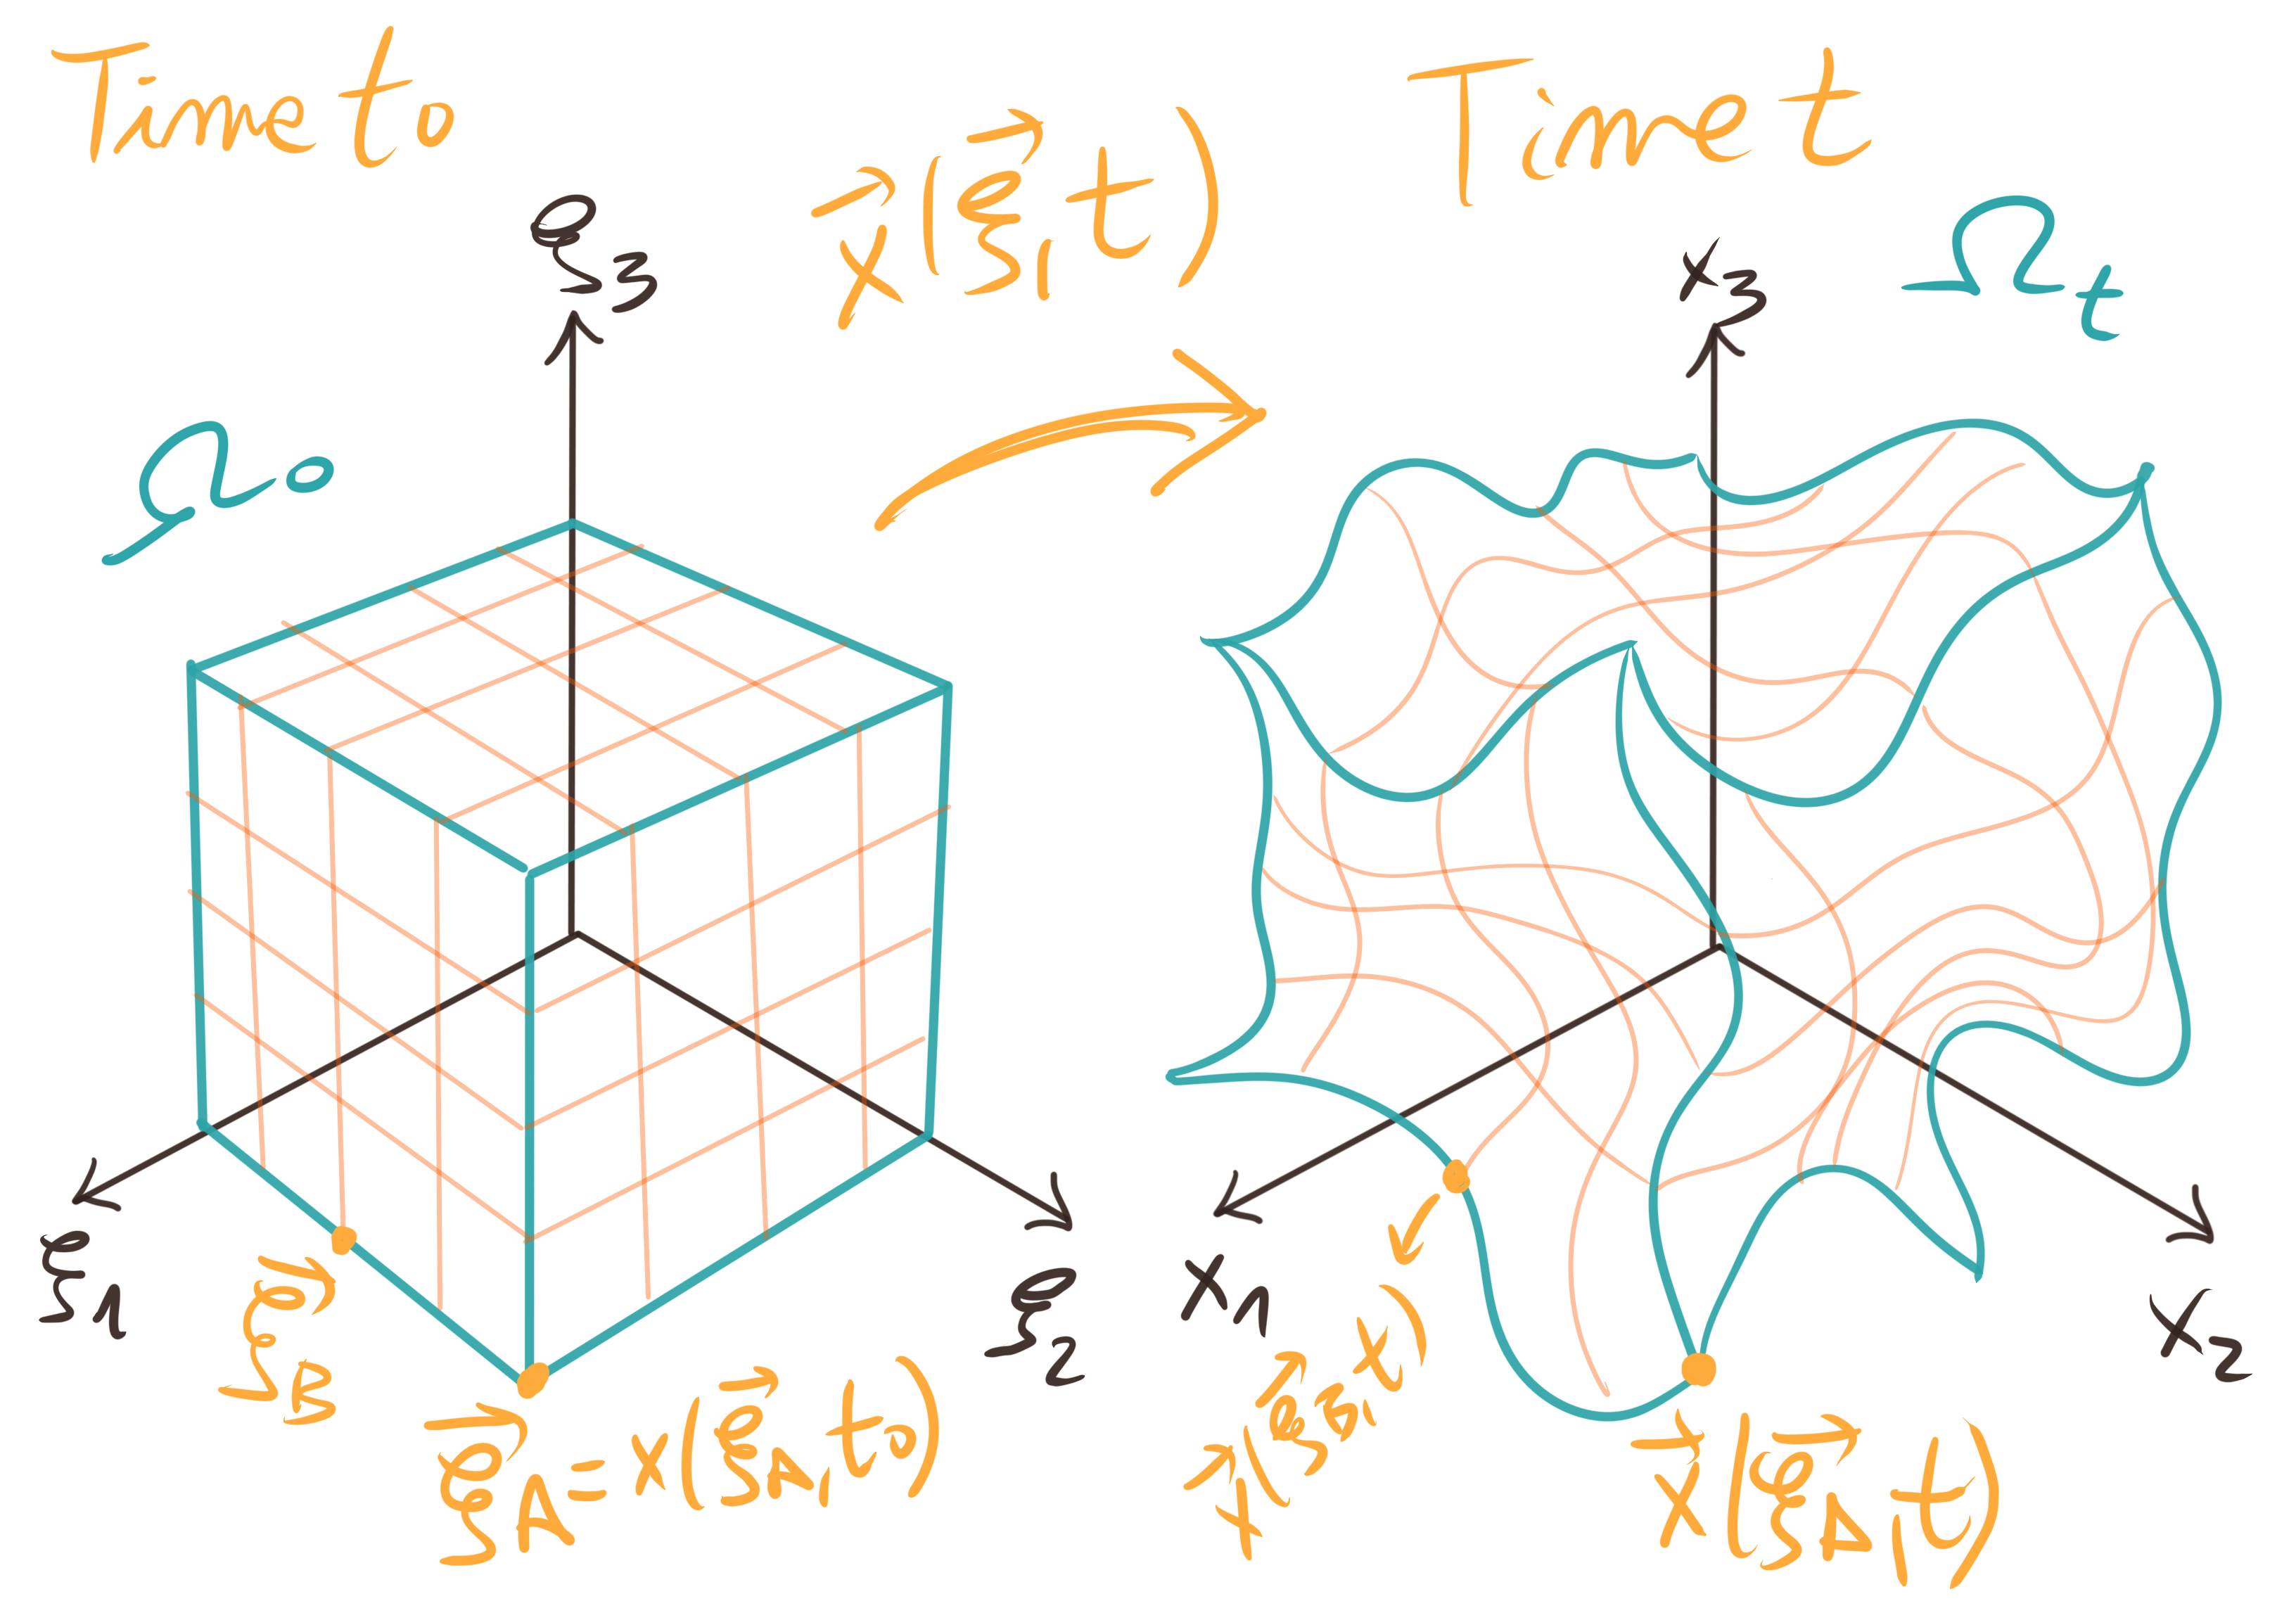
\includegraphics[width=0.57\linewidth]{1deforma.png}
  \caption{Depiction of the $N=3$ case of a homeomorphism representing the trajectory ensemble of a fluid following the notation presented in the text. \vspace{-0.2cm}}
  \label{fig:deform}
\end{figure}

We say that these alternative Universes are {\bf Tangent Universes}, because they can be arbitrarily close to each other in configuration space (that is, the set of positions in physical space for their particles can be arbitrarily similar), but their trajectories never cross each other, meaning they never have the same configuration at the same time.

\newpage
Note now that if we were just given the continuous velocity field for the trajectories of the Universes $\vec{v}\qty(\vec{x}(\vec{\xi},t),t):=\dv{\vec{x}(\vec{\xi},t)}{t}$, we could simply get the ensemble of trajectories by integration.

\begin{equation}
\vec{x}\qty(\vec{\xi},t)=\int_{t_0}^t \vec{v}\qty(\vec{x}(\vec{\xi},t),t)\ dt
\end{equation}
using the initial condition $\vec{x}\qty(\vec{\xi},t_0)=\vec{\xi}$ we have set by definition.

Thus, the velocity field seems to uniquely characterize the trajectory ensemble. This is why it will be one of the properties of the fluid we will look for when trying to define the state of the Tangent Universe Fluid.

There is yet another thing we need to assume to arrive to Quantum Mechanics. The relative amount of Universes in each configuration need not be homogeneous, meaning, we can define the ratio of Universes in a certain configuration, with respect to the total, as a (positive) density function $\rho(\vec{x},t)$, the {\bf density of tangent Universes}. Since we define it to be normalized with respect to the total number of Universes, we assume it integrates to unity in configuration space.

\begin{equation}
\iint_{\Omega_t} \rho(\vec{x},t)\ dx_1\cdots dx_N=1\quad \forall t
\end{equation}

Then, integrating this density in a certain volume $V\subseteq\R^N$ would give us the relative number of Universes with configurations in $V$, which by definition will be a positive real number in the range $[0,1]$.

These two fields in configuration space: the velocity of the trajectory ensemble $\vec{v}(\vec{x},t)$ (defining the ensemble $\vec{x}(\vec{\xi},t)$) and the relative tangent Universe density $\rho(\vec{x},t)$, will completely define the state of the Fluid of Universes at all times.

%\mybox{One could argue that we could also set additional or alternative epistemological or ontological bases, such as the velocity of the degrees of freedom of the Universe, their energy, or any other derived mathematical property. However, it turns out that if we are to measure the velocity of something, we always end up measuring the position of a cursor, even if the cursor was designed to be coupled or causally correlated with the velocity of the measured thing, or alternatively, we end up measuring the position of the thing in different close times and then dividing by the elapsed time increment. In fact, since position is also the ontological basis of classical mechanics, classically interesting properties in last resort are always defined using the position, meaning that in principle it seems that we can always compute properties of interest as derived from the position of the things.

%Note however that fixing the position as epistemological basis of the model does not restrict the ontological basis to be so: the true underlying basic essence of reality could be any other property of the system (as suggest the so called "modal theories"). However, since following the philosophical prologue, in practice there is almost no distinction between what we can consider to be real and the common human phenomenon. Thus, position of things in the phenomenon being so simple to agree on, it seems a reasonable ontology for a model.

%All in all, we choose as the measurable (epistemologically accesible) and underlying (ontological fabric) property, defining the state of our Universe, the space of possible configurations of the degrees of freedom of the Universe in each time. This is what we call the {\bf configuration space} of the Universe in each time.}

\subsection*{A.1.3. The Lagrangian and Eulerian Frames}
\addcontentsline{toc}{subsubsection}{1.3. The Lagrangian and Eulerian Frames}

We can now realize that we will be able to describe a state variable of the fluid, both by reference to a specific configuration-space position $\vec{x}$ at a certain time $t$ or by reference to a specific fluid element (or possible Universe) $\vec{\xi}$ at a certain time. These will be respectively the Eulerian and the Lagrangian frames. 

Given a property $f$ of the fluid (like the density, the velocity or any other derived one), it will be described in the Lagrangian frame if its values are given as seen from the $\vec{\xi}$-th Universe, that is, along the trajectory of that fluid element $f(\vec{x}(\vec{\xi},t),t)$. Alternatively, we could see the value of the properties at each time from a particular fixed Universe configuration $\vec{x}$, as $f(\vec{x},t)$, which would be the Eulerian frame.
 




 
\subsection*{A.1.4. The Measurement Axiom}

\addcontentsline{toc}{subsubsection}{1.4. The Measurement Axiom}
% Why QMs seem to be a non-deterministic theory, where in reality it is! (Since it can be formulated with only unitary deterministic time evolution!)

If we knew $\vec{\xi}\in\R^N$ was the position of every particle our Universe at an arbitrary single time, say at time $t_0$, we could then deterministically predict the time evolution of our Universe using the trajectory ensemble $\vec{x}(\vec{\xi},t)$. However, knowning the position of every particle in the Universe at the same time is far from being possible. Therefore, we cannot exactly know which of the tangent Universes is ours. From our point of view, the configuration of our Universe is thus an unknown, a random variable. 

Since a priori, we have no information about which of the Universes is ours, we can refer to the tangent Universes as {\bf possible Universes}. A priori then, the best guess we can make is giving the same probability to each of the possible Universes to be ours. As the relative amount of Universes is given by the density $\rho(\vec{x},t)$, which we conveniently decided to normalize to unity, this would mean that we could identify the probability density of the configuration of our Universe with the density of tangent Universes (assigning a same probability to each possible Universe, we will have a weight due to their relative amount). That is, for a domain $V\subseteq \R^N$:
\begin{equation}
P\qty(\text{our Universe has its configuration in }V\text{ at time }t)=P(\vec{x}\in V\ |\ t) := \iint_{V}\rho(\vec{x},t)\ dx_1\cdots dx_N
\end{equation}

If instead we are only interested on the probability that a subset of the particles of our Universe $\vec{y}=(x_1,...,x_m)$ such that $m<N$, have their configuration in $V_y\subseteq \R^m$, we would simply use the marginal probability density derived from the global prior density:
$$
P(\vec{y}\in V_y\ |\ t) := \iint_{V_y}\qty(\iint_{\Omega_t}\rho(\vec{x},t)\ dx_{m+1}\cdots dx_N)dx_1\cdots dx_m
$$
\mybox{
Note that for the introduction of the narrative, we have been saying that ontologically our Universe has a discrete trajectory $\vec{x}(\vec{\xi},t)$, however, since in practice it is not possible to know the position of a particle with infinite precision (since we are dealing with continuous variables and not a variable with a countable support), the tangent Universes we should consider ontologically are those ones weighted by the density $\rho(\vec{\xi},t)$ and not the actual discrete ones. That is to say, the density of Universes will not need to be preserved along the trajectories! This is just the discussion many authors have posed on the meaninglessness of observing a discrete value for a continuous probability density variable. We will see the relevance of this when we talk about the local conservation of the amount of Universes in the next section.\\

It is interesting however that this observation opens the question of whether quentum theory is just the continous limit of a more fundamental theory where there is actually a countably infinite number of possible Universes! If their number is very big, most predictions would coincide at a big degree with the theory were there is an uncountable number of Universes. However, they could clearly have different predictions for some very fine experiments. Different predictions that could be perceived in the phenomenon and thus help falsify the underlying theory. It is here where we can see the relevance of a narrative given to a physical theory. It can open ways to search for alternative theories and test non-trivial limits of the theory. Actually, such an alternative Discrete Tangent Universe Quantum Theory was discussed very recently in Ref. \cite{TangentWiseman} by Wiseman et al.
}

\newpage
\fancyhead[R]{\em The Dynamics of the Universe}
\section*{A.2. The Dynamics of the Universe}
\addcontentsline{toc}{subsection}{2. The Dynamics of the Universe}
% Las ecuaciones dinámicas de la densidad y de la acción. La ecuación de Schrödinger

\subsection*{A.2.1. The Quantum Action Principle}

\addcontentsline{toc}{subsubsection}{2.1. The Quantum Action Principle}

\subsection*{A.2.2. The Dynamics of the Density of Universes}

\addcontentsline{toc}{subsubsection}{2.2. The Dynamics of the Density of Universes}


\subsection*{A.2.3. The Dynamics of the Action Density}

\addcontentsline{toc}{subsubsection}{2.3. The Dynamics of the Action Density}

\subsection*{A.2.4. The Dynamics of The Wavefuntion}

\addcontentsline{toc}{subsubsection}{2.4. The Dynamics of The Wavefunction}


\newpage
\fancyhead[R]{\em The State of a Partition of the Universe}
\section*{A.3. The State of a Partition of the Universe}
\addcontentsline{toc}{subsection}{ 3. The State of a Partition of the Universe}
% Azaldu la función de onda efectiva y la conditional wave-function

\subsection*{A.3.1. The Epistemology of the Model}
\addcontentsline{toc}{subsubsection}{3.1. The Epistemology of the Model}
% Lo que se puede saber independientemente de la realidad subyacente

\subsection*{A.3.2. An Effective Wavefunction}

\addcontentsline{toc}{subsubsection}{3.2. An Effective Wavefunction}

\subsection*{A.3.3. The Conditional Wavefunction}

\addcontentsline{toc}{subsubsection}{3.3. The Conditional Wavefunction}

\newpage
\begin{kapituloBerria}{Part B}{" Measuring a Quantum System means knowing\\ the state of the system after the measurement, with\\ probabilities due to the state before the measurement."}
The Measurement 
\end{kapituloBerria}
\newpage
\fancyhead[L]{\null}
\fancyhead[R]{\null}
\null
\clearpage

\fancyhead[L]{The Measurement}

\fancyhead[R]{\em The Von Neumann Chain and Perturbing the System}
\section*{B.1. The Von Neumann Chain and Perturbing the System}
\addcontentsline{toc}{section}{Part B: The Measurement}
\addcontentsline{toc}{subsection}{1. The Von Neumann Chain and Perturbing the System}

\fancyhead[R]{\em The Apparently Collapsing Measurement}
\section*{B.2. The Apparently Collapsing Measurement}
\addcontentsline{toc}{subsection}{2. The Apparently Collapsing Measurement}

\subsection*{B.2.1. Discrete Spectrum Measurement}
\addcontentsline{toc}{subsubsection}{2.1. Discrete Spectrum Measurement}
\subsection*{B.2.2. Continuous Spectrum Measurement}
\addcontentsline{toc}{subsubsection}{2.2. Continuous Spectrum Measurement}

\fancyhead[R]{\em The Generalized Measurement}
\section*{B.3. The Generalized Measurement}
\addcontentsline{toc}{subsection}{3. The Generalized Measurement}

\subsection*{B.3.1. A Strong Measurement}
\addcontentsline{toc}{subsubsection}{3.1. A Strong Measurement}
\subsection*{B.3.2. A Weak Measurement}
\addcontentsline{toc}{subsubsection}{3.2. A Weak Measurement}

\fancyhead[R]{\em Properties of the Wavefunction vs Properties of the Trajectory}
\section*{B.4. Properties of the Wavefunction vs Properties of the Trajectory}
\addcontentsline{toc}{subsection}{4.  Properties of the Wavefunction vs Properties of the Trajectory}

\subsection*{B.4.1 The In Position Weak Values as Trajectory Properties}
\addcontentsline{toc}{subsubsection}{4.1. The Weak Values}

\newpage



\newpage
\begin{kapituloBerria}{Part C}{" A wavefunction keeps track of\\ Tangent Universes while a Density Matrix\\ keeps track of Parallel Wavefunctions."}
The Density Matrix 
\end{kapituloBerria}
\newpage
\null
\fancyhead[L]{\null}
\fancyhead[R]{\null}
\clearpage

\fancyhead[L]{The Density Matrix}

\fancyhead[R]{\em The Way to Keep Track of Parallel Realities}
\section*{C.1. The Way to Keep Track of Parallel Realities}

\addcontentsline{toc}{section}{Part C: The Density Matrix}
\addcontentsline{toc}{subsection}{1. The Way to Keep Track of Parallel Realities}

\fancyhead[R]{\em The Reduced Density Matrix}
\section*{C.2. The Reduced Density Matrix}
\addcontentsline{toc}{subsection}{2. The Reduced Density Matrix}

\fancyhead[R]{\em  The Unconditional Measurement and the Choice of Basis}
\section*{C.3. The Unconditional Measurement and the Choice of Basis}
\addcontentsline{toc}{subsection}{3. The Unconditional Measurement and the Choice of Basis}

\fancyhead[R]{\em  Pure Unravellings}
\section*{C.4. Pure Unravellings}
\addcontentsline{toc}{subsection}{4. Pure Unravellings}



\fancyhead[R]{\em  Pure Unravellings}
\section*{C.5. Complete Positive Maps: Any Quantum Operation is a Measurement}\addcontentsline{toc}{subsection}{5.  Complete Positive Maps: Any Quantum Operation is a Measurement}
% Explicar lo que es la operacion mas general que se le puede hacer a un state y ver que siempre se puede ver como una measurement con el Naimark Theorem


\fancyhead[R]{\em  Pure Unravellings}
\section*{C.6. Noise, Decoherence and the Environment}\addcontentsline{toc}{subsection}{6. Noise, Decoherence and the Environment}
% Zelan noise beti al dozun ulertu como una measurement realizada en el entorno, aka coupling and decoupling del entorno y el systema after unitary etc.


\begin{kapituloBerria}{Part D}{" The Quantum Measurement and the Decohering Noise have\\ exactly the same mathematical formulation. Are they the same thing?"}
Markovianity and\\ Master Equations
\end{kapituloBerria}
\newpage
\fancyhead[L]{\null}
\fancyhead[R]{\null}
\null
\clearpage

\fancyhead[L]{Markovianity and Master Equations}

\fancyhead[L]{Markovianity and Master Equations}
\section*{D.1. Some Possible Quantum Markovianity Definitions}

\addcontentsline{toc}{section}{Part D: Markovianity and Master Equations}
\addcontentsline{toc}{subsection}{1. Some Possible Quantum Markovianity Definitions}

\subsection*{D.1.1. Past-Future Independence}\addcontentsline{toc}{subsubsection}{1.1. Past-Future Independence}

\subsection*{D.1.2. Etc.}\addcontentsline{toc}{subsubsection}{1.2. Etc.}


\fancyhead[R]{\em  Continuous Measurements}
\section*{D.2. Continuous Measurements:\\ Introduction to Master and Stochastic Schrödinger Equations}\addcontentsline{toc}{subsection}{2. Continuous Measurements: Introduction to Master and Stochastic Schrödinger Equations}

\fancyhead[R]{\em The Lindblad Equations}
\section*{D.3. The Most General Markovian Master Equations:\\ The Lindblad Equations}\addcontentsline{toc}{subsection}{3. The Most General Markovian Master Equations: the Lindblad Equations}

\fancyhead[R]{\em Markovian Stochastic Schrödinger Equations}
\section*{D.4. Markovian Stochastic Schrödinger Equations:\\ Pure Unravellings}\addcontentsline{toc}{subsection}{4. Markovian Stochastic Schrödinger Equations: Pure Unravellings}

\fancyhead[R]{\em  The Nakajima-Zwanzig Equation}
\section*{D.5. The Most General non-Markovian Master Equation:\\ The Nakajima-Zwanzig Equation}\addcontentsline{toc}{subsection}{5. The Most General non-Markovian Master Equation: the Nakajima-Zwanzig Equation}


\fancyhead[R]{\em Non-Markovian Stochastic Schrödinger Equations}
\section*{D.6. Non-Markovian Stochastic Schrödinger Equations:\\ the Conditional Wavefunction}
\addcontentsline{toc}{subsection}{6. Non-Markovian Stochastic Schrödinger Equations: the Conditional Wavefunction}

\subsection*{D.6.1 Wiseman's}
\addcontentsline{toc}{subsubsection}{6.1. Wiseman's}

\subsection*{D.6.2 Ours}\addcontentsline{toc}{subsubsection}{6.2. Ours}
% Guk eztogu en el interaction frame consideretan sino ke en general. Asike azaldu zelan al dan gure cwfakaz rekonstruidu la full reduced density adibidez ta gero redirigidu nire tratadoko part Lagrangian part Eulerian kapitulora!





\newpage
 
\fancyhead[R]{\em References}
\fancyhead[L]{\null}


\begin{thebibliography}{1}
\addcontentsline{toc}{section}{References}

% Cita a la Crítica a la Razón Pura de Kant.

% Cita a la Mind and Matter de Schrödinger.



%\bibitem{Albareda}
%	Albareda G, Kelly A, Rubio A. {\em Nonadiabatic quantum dynamics without potential energy surfaces.} Phys Rev Materials. 2019; 3: 023803. 

	
\end{thebibliography}


\end{document}
